\documentclass[12pt,a4paper]{article}
\usepackage{cmap} % Makes the PDF copiable. See http://tex.stackexchange.com/a/64198/25761
\usepackage[T1]{fontenc}
\usepackage[brazil]{babel}
\usepackage[utf8]{inputenc}
\usepackage{amsmath}
\usepackage{amsfonts}
\usepackage{amssymb}
\usepackage{amsthm}
\usepackage{textcomp} % \degree
\usepackage{gensymb} % \degree
\usepackage[usenames,svgnames,dvipsnames]{xcolor}
\usepackage{hyperref}
\usepackage{multicol}
\usepackage{graphicx}
\usepackage[margin=2cm]{geometry}
\usepackage{systeme}

\hypersetup{
    colorlinks = true,
    allcolors = {blue}
}

% TODO: Consider using exsheets
% http://linorg.usp.br/CTAN/macros/latex/contrib/exsheets/exsheets_en.pdf
%
% http://ctan.org/tex-archive/macros/latex/contrib/exercise/
% Options: answerdelayed,lastexercise,noanswer
\usepackage[answerdelayed,lastexercise]{exercise}

\addto\captionsbrazil{%
\def\listexercisename{Lista de exerc\'icios}%
\def\ExerciseName{Exerc\'icio}%
\def\AnswerName{Solu\c{c}\~ao do exerc\'icio}%
\def\ExerciseListName{Ex.}%
\def\AnswerListName{Solu\c{c}\~ao}%
\def\ExePartName{Parte}%
\def\ArticleOf{de\ }%
}

\renewcommand{\ExerciseHeaderTitle}{(\ExerciseTitle)\ }
\renewcommand{\ExerciseListHeader}{%\ExerciseHeaderDifficulty%
\textbf{%\ExerciseListName\
\ExerciseHeaderNB.\ %
%\ --- \
\ExerciseHeaderTitle}%
%\ExerciseHeaderOrigin
\ignorespaces}
\renewcommand{\AnswerListHeader}{\textbf{\ExerciseHeaderNB.\ (\AnswerListName)\ }}

\newcommand{\fixme}{{\color{red}(...)}}
\newcommand*\R{\mathbb{R}}

% Loop Space / CC BY-SA-3.0 / https://tex.stackexchange.com/a/2238/25761
\newenvironment{amatrix}[1]{%
  \left[\begin{array}{@{}*{#1}{c}|c@{}}
}{%
  \end{array}\right]
}

% Loop Space / CC BY-SA-3.0 / https://tex.stackexchange.com/a/3164/25761
%--------grstep
% For denoting a Gauss' reduction step.
% Use as: \grstep{\rho_1+\rho_3} or \grstep[2\rho_5 \\ 3\rho_6]{\rho_1+\rho_3}
\newcommand{\grstep}[2][\relax]{%
   \ensuremath{\mathrel{
       {\mathop{\longrightarrow}\limits^{#2\mathstrut}_{
                                     \begin{subarray}{l} #1 \end{subarray}}}}}}

\renewcommand{\theenumi}{\alph{enumi}}
\renewcommand\labelenumi{(\theenumi) }

\newcommand*\tipo{Prova IV}
\newcommand*\turma{NEX162-C}
\newcommand*\disciplina{ALI0001}
\newcommand*\eu{Helder G. G. de Lima}
\newcommand*\data{06/12/2016}

\author{\eu}
\title{\tipo - \disciplina}
\date{\data}

\begin{document}
\thispagestyle{empty}
\newgeometry{margin=2cm,bottom=0.5cm}
\begin{center}

\includegraphics[width=9.0cm]{marca} \\
\textbf{\tipo\ (\disciplina / \turma)} \\
Prof. \eu\footnote{
Este é um material de acesso livre distribuído sob os termos da licença \href{https://creativecommons.org/licenses/by-sa/4.0/deed.pt_BR}{Creative Commons Atribuição-CompartilhaIgual 4.0 Internacional}}
\end{center}

\noindent Nome do(a) aluno(a): \underline{\hspace{9,7cm}} Data: \underline{\data}

%\section*{Instruções}
\begin{center}\fbox{
\begin{minipage}{14cm}

{\footnotesize
\begin{itemize}
\renewcommand{\theenumi}{\Roman{enumi}}
\item Identifique-se em todas as folhas.
\item Mantenha o celular e os demais equipamentos eletrônicos desligados durante a prova.
\item Escolha os itens a resolver de modo a totalizar até 10,0 pontos.
\end{itemize}
}

\end{minipage}
}
\end{center}

%\section*{Questões}
\begin{ExerciseList}

\Exercise[title={2,5}] Suponha que um operador linear $T: \R^2 \to \R^2$ transforma os pontos indicados na \autoref{fig:dom} nos pontos correspondentes da \autoref{fig:cd}:
\begin{figure}[h]
    \centering
    \begin{minipage}{0.45\textwidth}
        \centering
        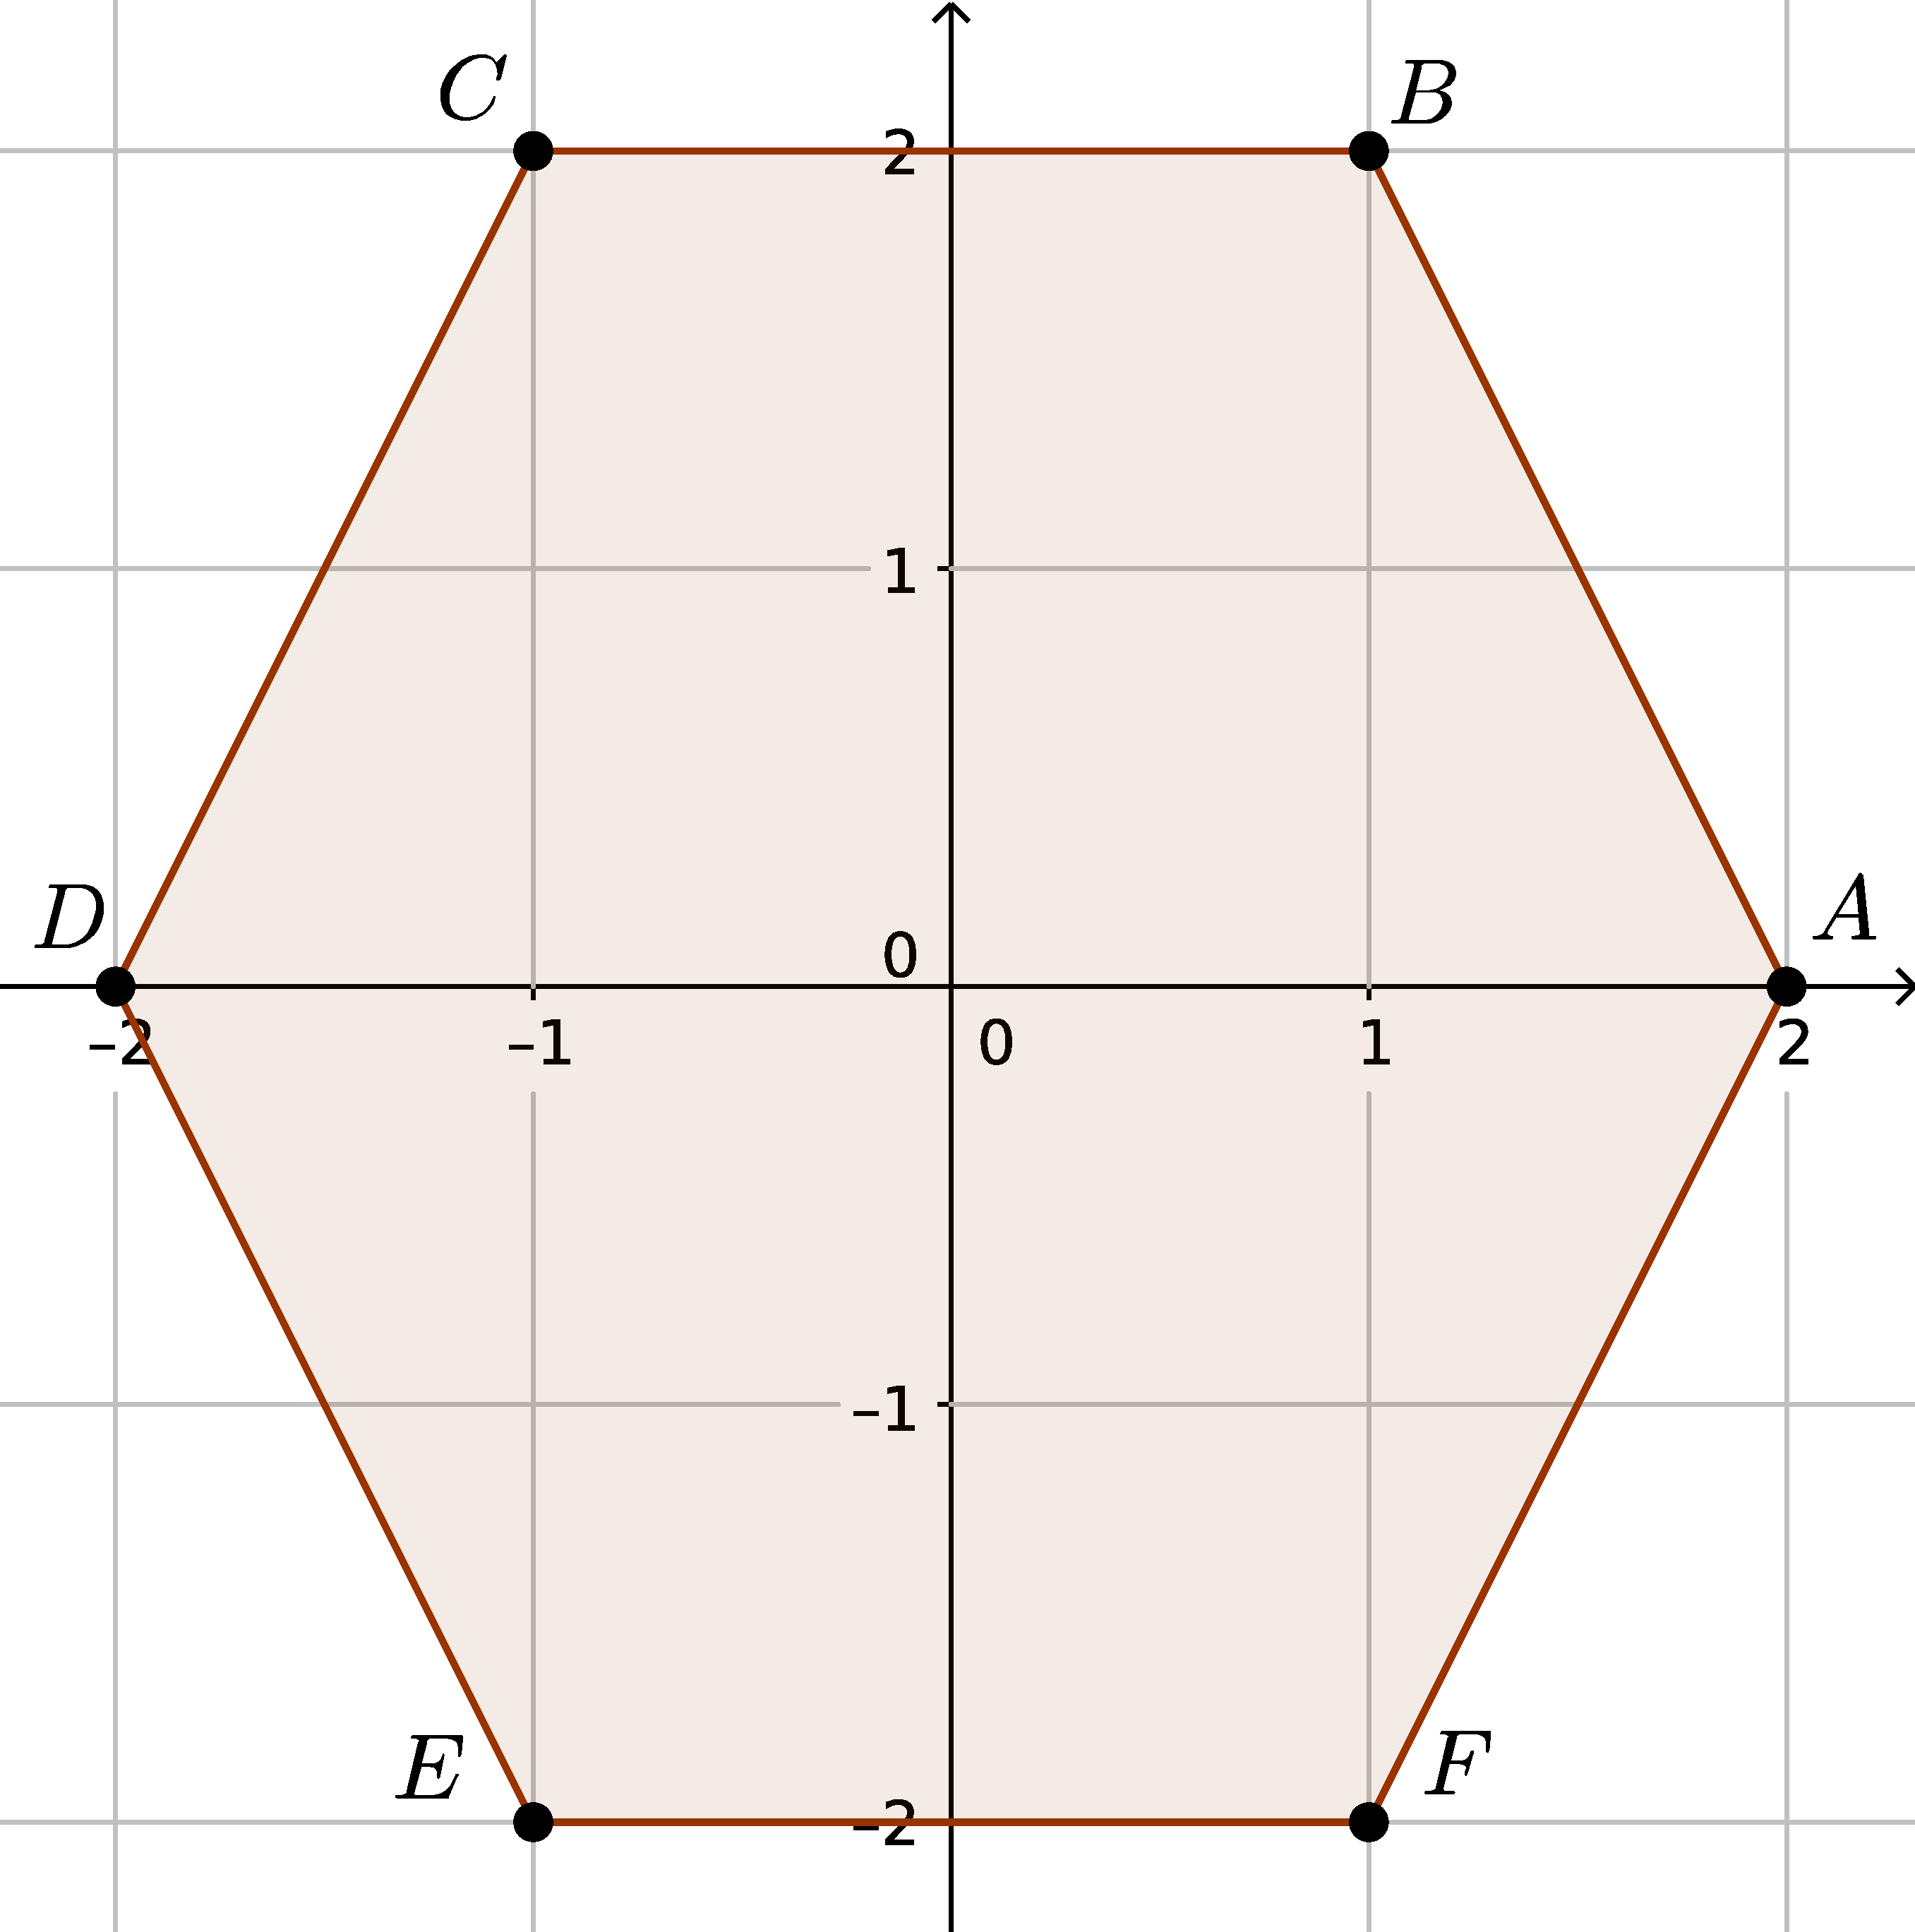
\includegraphics[height=0.48\textwidth]{img/prova-4-nex-hexagono-dom}
        \caption{Domínio}\label{fig:dom}
    \end{minipage}\hfill
    \begin{minipage}{0.45\textwidth}
        \centering
        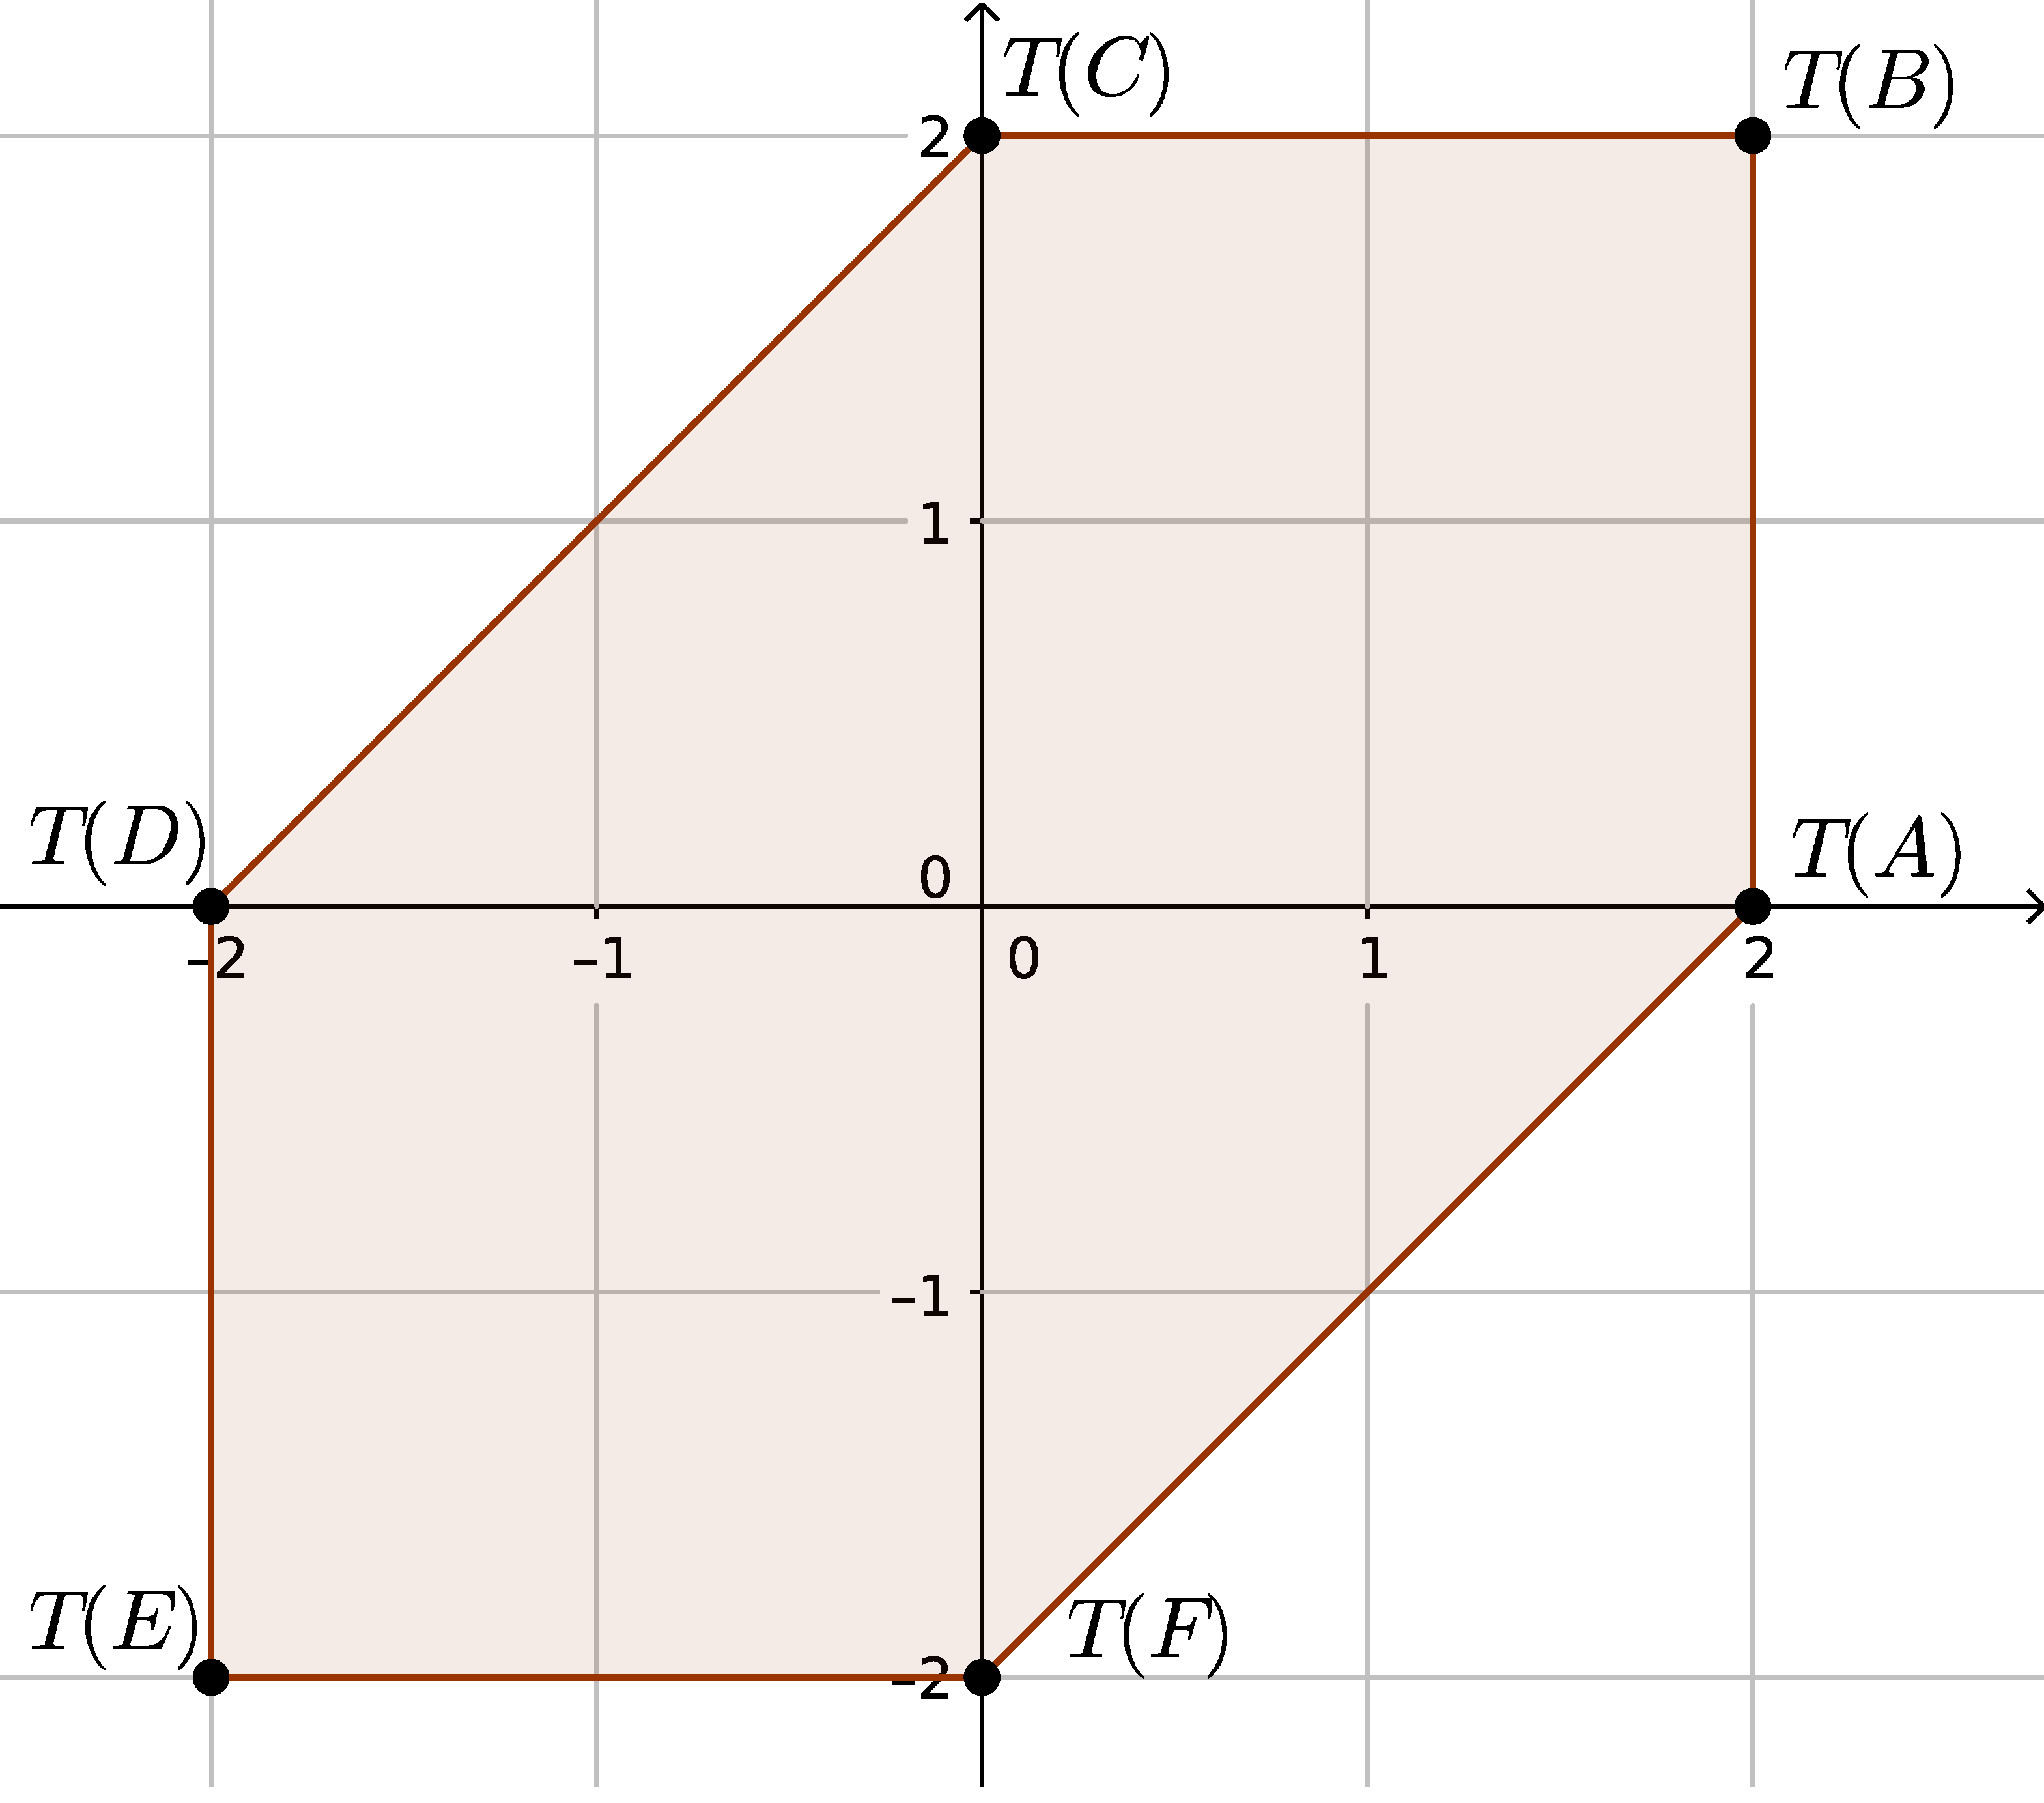
\includegraphics[height=0.48\textwidth]{img/prova-4-nex-hexagono-img}
        \caption{Contradomínio}\label{fig:cd}
    \end{minipage}
\end{figure}
\begin{enumerate}
\item Qual é a fórmula para $T(x,y)$?
\item Quais são os autovalores e os autovetores de $T$?
\end{enumerate}
\Answer \fixme

\Exercise[title={2,5}]
Se $A$ e $B$ são matrizes quadradas, dizemos que \textbf{$A$ é semelhante a $B$} se existe (pelo menos) uma matriz inversível $P$ tal que $A = P^{-1} B P$. Mostre que:
\begin{enumerate}
\item Toda matriz quadrada $A$ é semelhante a si mesma.
\item Sempre que $A$ é semelhante a $B$, a matriz $B$ também é semelhante à matriz $A$.
\item Sempre que $A$ é semelhante a $B$ e $B$ é semelhante a $C$, tem-se que $A$ é semelhante a $C$.
\end{enumerate}
\Answer \fixme

\Exercise[title={2,5}]
Seja $T: P_2 \to P_2$ a função definida por $T(q) = q^\prime$. Determine o(s) autovalor(es) e autovetores de $T$, e dimensão dos autoespaços associados. Com base nos resultados obtidos, pode-se afirmar que $T$ é diagonalizável? Explique.
\Answer \fixme

\Exercise[title={2,5}] Se $T : \R^2 \to \R^2$ é o operador linear dado por $T (x, y) = (9x - 3y, -3x + y)$, encontre uma base $\beta$ de $\R^2$ formada por autovetores de $T$ e mostre que a matriz $[T]_\beta^\beta$ de $T$ é diagonal.
\Answer \fixme

\Exercise[title={2,5}] Verifique se a matriz $A =
\begin{bmatrix}
1& 0& 0& 0\\
-1& 2& 0& 0\\
2& 0& 0& 0\\
1& 0& 0& 0
\end{bmatrix}$ é diagonalizável. Em caso afirmativo, obtenha uma matriz $P$ e uma matriz $D$ tais que $D = P^{-1} A P$ seja diagonal.
\Answer \fixme
\end{ExerciseList}

\begin{center}
BOA PROVA!
\end{center}

%\newpage
%\restoregeometry
%\section*{Respostas}
%\shipoutAnswer
\end{document}
